% Replaces the placeholder "[NEED TO DO CURVE FITTING ON T3 AND T4]" in Section 4.4.2
% Requires \usepackage{graphicx,subcaption,booktabs}

\subsubsection{Curve fitting of $T_3$ and $T_4$}
With the gains and $T_1$, $T_2$ fixed at the values above, $T_3$ and $T_4$ are
estimated by solving the two least-squares problems in Section~4.4.1 with
\texttt{lsqcurvefit}, using the lower bound $T>0$ and the initial guess
$T^{(0)} = 30$~s. The data are the deterministic normalized step responses
$S_{12}^{\text{meas}}(t_k)$ and $S_{21}^{\text{meas}}(t_k)$ for the $+10\%$ step,
sampled every $T_s = 10$~s over 20 minutes ($N=121$). The fit gives
\begin{equation}
    \hat{T}_3 \approx 48.7~\text{s}, \qquad \hat{T}_4 \approx 51.7~\text{s}.
\end{equation}
Figure~\ref{fig:curvefit_T3_T4} shows that the fitted second-order models are
almost indistinguishable from the nonlinear simulation. The residuals are of
order $10^{-5}$ (RMSE $1.6\cdot 10^{-5}$ and $3.8\cdot 10^{-5}$), compared with
gains of $K_{12}\approx 0.076$ and $K_{21}\approx 0.113$. The small, structured
residual during the initial transient comes from the nonlinearity of the
outflow $a_i\sqrt{2gh_i}$, which the linear model cannot capture.

The upper tanks respond roughly twice as fast as the lower tanks
($T_3, T_4 \approx 50$~s against $T_1, T_2 \approx 100$~s). This is expected,
since the time constant of a tank scales with $\sqrt{h_i}$ and the steady-state
levels of tanks 3 and 4 ($12$--$14$~cm) are much lower than those of tanks 1
and 2 ($46$--$57$~cm). Table~\ref{tab:T_vs_step} repeats the identification for
the larger steps. $\hat{T}_3$ and $\hat{T}_4$ hardly change, whereas $T_1$ and
$T_2$ grow by about $13\%$ for the $+50\%$ step. This confirms that the
$+10\%$ step gives the estimates closest to the operating point. The estimates
also agree well with the time constants of the linearized model,
$T_i = (A_i/a_i)\sqrt{2h_{i,s}/g}$.

\begin{figure}[htbp]
    \centering
    \begin{subfigure}[b]{0.49\textwidth}
        \centering
        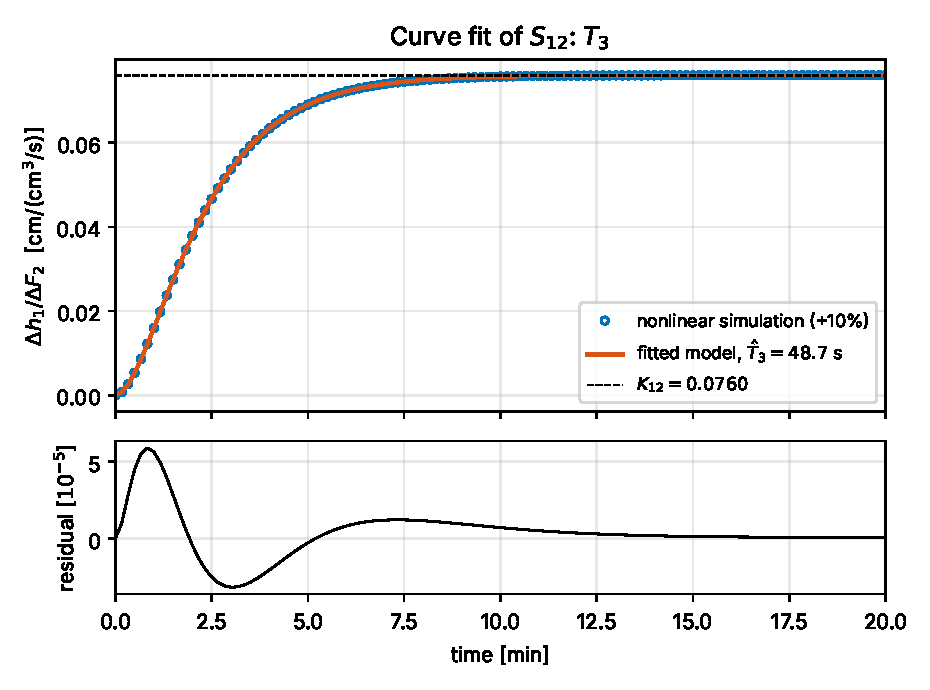
\includegraphics[width=\textwidth]{plots/sim_4_4_curvefit_T3.pdf}
        \caption{$S_{12}$ (input $F_2$, output $h_1$): fit of $T_3$.}
        \label{fig:curvefit_T3}
    \end{subfigure}
    \hfill
    \begin{subfigure}[b]{0.49\textwidth}
        \centering
        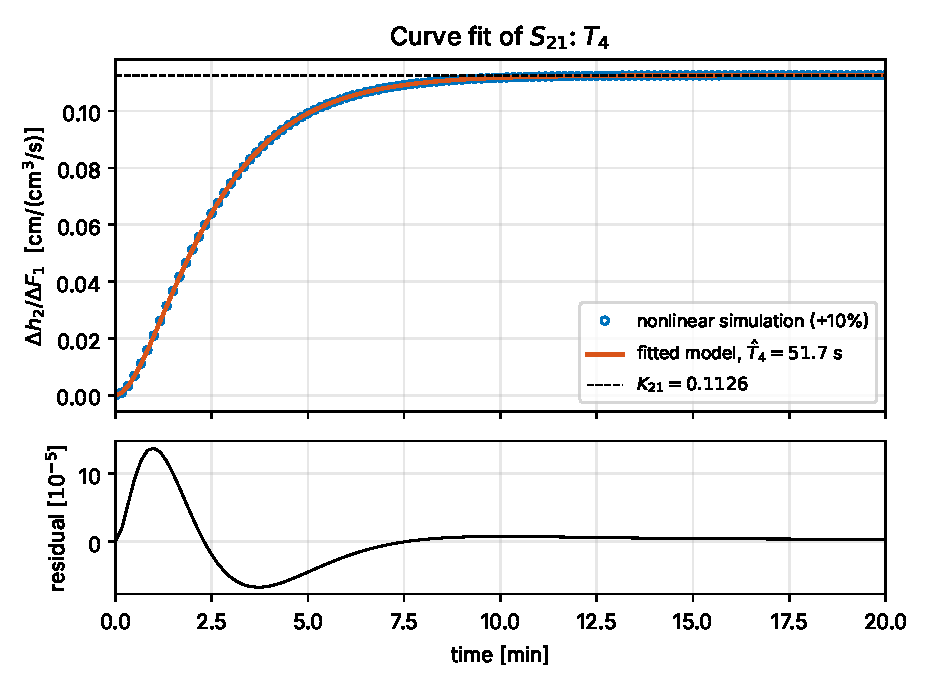
\includegraphics[width=\textwidth]{plots/sim_4_4_curvefit_T4.pdf}
        \caption{$S_{21}$ (input $F_1$, output $h_2$): fit of $T_4$.}
        \label{fig:curvefit_T4}
    \end{subfigure}
    \caption{Least-squares fit of the second-order step responses to the
    deterministic normalized step responses for a $+10\%$ step. Top: nonlinear
    simulation (circles) and fitted model (line). Bottom: residuals.}
    \label{fig:curvefit_T3_T4}
\end{figure}

\begin{table}[htbp]
    \centering
    \caption{Time constants identified for each step size, compared with the
    linearized model.}
    \label{tab:T_vs_step}
    \begin{tabular}{lcccc}
        \toprule
        Step & $T_1$ [s] & $T_2$ [s] & $\hat{T}_3$ [s] & $\hat{T}_4$ [s] \\
        \midrule
        $+10\%$          & 98.4  & 109.2 & 48.7 & 51.7 \\
        $+25\%$          & 103.3 & 114.9 & 48.5 & 52.1 \\
        $+50\%$          & 111.3 & 124.3 & 48.2 & 52.8 \\
        \midrule
        Linearized model & 95.2  & 105.5 & 48.9 & 51.5 \\
        \bottomrule
    \end{tabular}
\end{table}
